\documentclass[aspectratio=169,12pt]{beamer}
\usepackage{amsmath}
\usepackage{amssymb}
\usepackage[most]{tcolorbox}
\usepackage{tikz}
\usepackage{graphicx}
\usepackage[sfdefault,lf]{FiraSans}
\renewcommand{\familydefault}{\sfdefault}
\setlength{\parindent}{0pt}
\everymath{\displaystyle}

\setbeamertemplate{navigation symbols}{}
\setbeamertemplate{footline}{}
\setbeamertemplate{headline}{}

\definecolor{mmpageWhite}{HTML}{FCFBF7}
\definecolor{mmtanSoft}{HTML}{F7F5EF}
\definecolor{mmgreenDeep}{HTML}{244B2C}
\definecolor{mmgreenLeaf}{HTML}{5D8A56}
\definecolor{mmgreenSoft}{HTML}{E4EFD9}
\definecolor{mmtext}{HTML}{163221}

\setbeamercolor{background canvas}{bg=mmpageWhite}
\setbeamercolor{normal text}{fg=mmtext,bg=mmpageWhite}

\newtcolorbox{MMProblemCard}[1][]{enhanced,breakable=false,colback=white,colframe=black,boxrule=1.0pt,arc=5pt,left=3pt,right=3pt,top=2pt,bottom=2pt,before skip=0pt,after skip=0pt,height=0.26\textheight,valign=top,#1}
\newcommand{\KoruIcon}{\raisebox{-0.2em}{
\includegraphics[height=1.05em]{../../SITE/header-logo.png}}}
\newcommand{\HoeIcon}{\raisebox{-0.2em}{
\includegraphics[height=1.05em]{../../SITE/hoe.png}}}
\newcommand{\ScaffoldIcons}[1]{\ifcase#1\or \HoeIcon\or \HoeIcon\hspace{0.22em}\KoruIcon\or \KoruIcon\hspace{0.22em}\KoruIcon\hspace{0.22em}\KoruIcon\fi}
\newcommand{\WorksheetTitle}[2]{%
  {\colorbox{mmtanSoft}{\parbox[c][2.0em][c]{0.975\linewidth}{%
    \hspace{0.25em}{\Large\bfseries\textcolor{mmgreenDeep}{#1}\hfill\ScaffoldIcons{#2}}}}
  \par\vspace{0.08em}{\color{mmgreenLeaf}\rule{\linewidth}{2.0pt}}\par\vspace{0.04em}}
}
\newcommand{\MMProblem}[2]{\begin{MMProblemCard}\raggedright\small\textbf{#1.} #2\par\end{MMProblemCard}}

\setbeamertemplate{background}{
 \begin{tikzpicture}[remember picture,overlay]
 \draw[black,line width=1.5pt,rounded corners=10pt]
 ([xshift=0.45cm,yshift=-0.45cm]current page.north west)
 rectangle
 ([xshift=-0.45cm,yshift=0.45cm]current page.south east);
 \end{tikzpicture}
}

% Default worksheet generation rules:
% use notes-style beamer pages
% use bordered cards for individual problems
% target 9 problems per frame in a 3x3 grid
% target 3 frames per scaffold by default where content allows

\begin{document}\begin{frame}[t]
\WorksheetTitle{Push Tasks}
\vspace{-0.18em}
\begin{columns}[T,onlytextwidth]
\begin{column}{0.32\textwidth}\MMProblem{1}{Find \mbox{$x$} and then give all eight angle sizes.\\[0.4em]
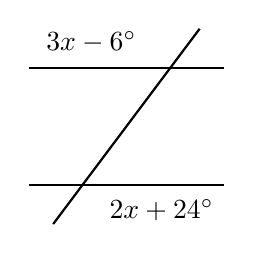
\begin{tikzpicture}[scale=0.62,baseline=(current bounding box.center)]
\draw[thick] (-2,1.2)--(2,1.2);
\draw[thick] (-2,-1.2)--(2,-1.2);
\draw[thick] (-1.5,-2)--(1.5,2);
\node[fill=white,inner sep=1pt] at (-0.72,1.72) {$3x-6^\circ$};
\node[fill=white,inner sep=1pt] at (0.72,-1.72) {$2x+24^\circ$};
\end{tikzpicture}}\end{column}
\begin{column}{0.32\textwidth}\MMProblem{2}{Find \mbox{$y$} and then state the acute angle size.\\[0.4em]
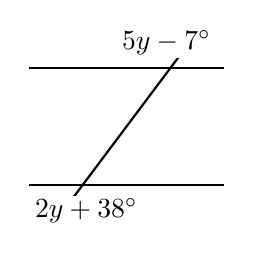
\begin{tikzpicture}[scale=0.62,baseline=(current bounding box.center)]
\draw[thick] (-2,1.2)--(2,1.2);
\draw[thick] (-2,-1.2)--(2,-1.2);
\draw[thick] (-1.5,-2)--(1.5,2);
\node[fill=white,inner sep=1pt] at (0.82,1.72) {$5y-7^\circ$};
\node[fill=white,inner sep=1pt] at (-0.82,-1.72) {$2y+38^\circ$};
\end{tikzpicture}}\end{column}
\begin{column}{0.32\textwidth}\MMProblem{3}{Find \mbox{$a$}. Then say whether \mbox{$4a+8^\circ$} is acute or obtuse.\\[0.4em]
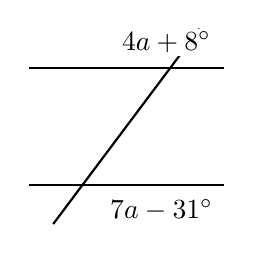
\begin{tikzpicture}[scale=0.62,baseline=(current bounding box.center)]
\draw[thick] (-2,1.2)--(2,1.2);
\draw[thick] (-2,-1.2)--(2,-1.2);
\draw[thick] (-1.5,-2)--(1.5,2);
\node[fill=white,inner sep=1pt] at (0.82,1.72) {$4a+8^\circ$};
\node[fill=white,inner sep=1pt] at (0.72,-1.72) {$7a-31^\circ$};
\end{tikzpicture}}\end{column}
\end{columns}
\vspace{0.45em}
\begin{columns}[T,onlytextwidth]
\begin{column}{0.32\textwidth}\MMProblem{4}{Two co-interior angles are \mbox{$(6m+4)^\circ$} and \mbox{$(3m+14)^\circ$}. Find \mbox{$m$} and both angles.}\end{column}
\begin{column}{0.32\textwidth}\MMProblem{5}{Two corresponding angles are \mbox{$(4p+9)^\circ$} and \mbox{$(2p+45)^\circ$}. Find \mbox{$p$}.}\end{column}
\begin{column}{0.32\textwidth}\MMProblem{6}{Two alternate angles are \mbox{$(5q-11)^\circ$} and \mbox{$(3q+27)^\circ$}. Find \mbox{$q$}.}\end{column}
\end{columns}
\vspace{0.45em}
\begin{columns}[T,onlytextwidth]
\begin{column}{0.32\textwidth}\MMProblem{7}{A pair of corresponding angles is \mbox{$124^\circ$} and \mbox{$124^\circ$}. Explain why that is evidence the lines are parallel.}\end{column}
\begin{column}{0.32\textwidth}\MMProblem{8}{A pair of co-interior angles is \mbox{$97^\circ$} and \mbox{$83^\circ$}. What conclusion can you make about the lines, and why?}\end{column}
\begin{column}{0.32\textwidth}\MMProblem{9}{A student writes: if two alternate angles add to \mbox{$180^\circ$}, the lines are parallel. Explain the mistake.}\end{column}
\end{columns}
\end{frame}
\begin{frame}[t]
\WorksheetTitle{Push Tasks}
\vspace{-0.18em}
\begin{columns}[T,onlytextwidth]
\begin{column}{0.32\textwidth}\MMProblem{1}{The acute angle is three times smaller than the obtuse angle. Find both angle sizes.}\end{column}
\begin{column}{0.32\textwidth}\MMProblem{2}{The obtuse angle is \mbox{$18^\circ$} bigger than twice the acute angle. Find both angle sizes.}\end{column}
\begin{column}{0.32\textwidth}\MMProblem{3}{Write two different facts you can prove once you know one angle is \mbox{$67^\circ$}.}\end{column}
\end{columns}
\vspace{0.45em}
\begin{columns}[T,onlytextwidth]
\begin{column}{0.32\textwidth}\MMProblem{4}{Explain the difference between corresponding angles and co-interior angles using the words \textit{position} and \textit{sum}.}\end{column}
\begin{column}{0.32\textwidth}\MMProblem{5}{Create your own short parallel-lines problem involving one unknown, then solve it.}\end{column}
\begin{column}{0.32\textwidth}\MMProblem{6}{}\end{column}
\end{columns}
\vspace{0.45em}
\begin{columns}[T,onlytextwidth]
\begin{column}{0.32\textwidth}\MMProblem{7}{}\end{column}
\begin{column}{0.32\textwidth}\MMProblem{8}{}\end{column}
\begin{column}{0.32\textwidth}\MMProblem{9}{}\end{column}
\end{columns}
\end{frame}
\end{document}
